\section{Color centers and broken bonds}\label{sec:16.6}

A fluorine atom knocked off its site in lithium fluoride leaves an anion vacancy, and an anion vacancy that binds an electron is an F center, which absorbs light near \SI{5.1}{eV}~\cite{guerreroperez2025first}. A dark-matter particle of \SI{0.5}{GeV} can give a fluorine nucleus at most \SI{188}{eV} (\cref{eq:1.3-ERmax}), a few times the tens of eV that a displacement costs. A molecule struck on one of its atoms comes apart in the same way when the kick exceeds its bond energy, \SI{4.75}{eV} for H$_2$. The F center and the broken molecule both persist, both lie in a crystal transparent to the light that reads them, and both can be counted singly. Budnik, Cheshnovsky, Slone and Volansky proposed color centers as a target for sub-GeV dark matter~\cite{budnik2018direct}, and Essig, Mardon, Slone and Volansky the breaking of chemical bonds~\cite{essig2017detection}.

\subsection{The color-center creation rate}\label{sec:16.6-cc}

A color center forms after the prompt window of \cref{sec:8.7}. Within that window, a femtosecond after the kick, the struck nucleus moves with the momentum it received and its neighbors have not yet responded; the class $\Lambda$ is a recoil of species $\kappa$ with energy deposit $\omega$ along $\hat{\vect{q}}$. The defect forms during the collision cascade that follows, within picoseconds, and its fate is decided later still, when the close pair recombines or does not and when the vacancy captures an electron or does not. The rate of creating readable centers is therefore the hand-off formula \cref{eq:8.7-handoff} with the cascade distribution $P_{\mathrm{casc}}(N_{\mathrm{eh}}|\Lambda)$ replaced by the probability $Y_{\mathrm{CC}}(\Lambda)$ that a seed of class $\Lambda$ ends as a center that the readout registers. \Cref{sec:18.3} makes precise how a recoil seeds the cascade, and \cref{sec:19.4} treats the energy that defects store. The conditions of \cref{sec:8.7} apply directly: the yield depends on the direction of the recoil relative to the crystal axes, so $\hat{\vect{q}}$ must stay inside the class sum, and a rate averaged over directions before the yield is applied is wrong near threshold.

The yield is a product of four probabilities, each fixed at a different stage:
\begin{equation}
  Y_{\mathrm{CC}}(E_R,\hat{\vect{r}}_R) = p_{\mathrm{FP}}(E_R,\hat{\vect{r}}_R)\;p_{\mathrm{surv}}\;p_q\;f_{\mathrm{opt}} .
  \label{eq:16.6-yield}
\end{equation}
The first, $p_{\mathrm{FP}}$, is the probability that a nucleus set moving with kinetic energy $E_R$ along $\hat{\vect{r}}_R$ leaves a Frenkel pair once the collision has died out. Its lowest crossing is the displacement threshold $E_{\mathrm{d}}(\hat{\vect{r}}_R)$ of \cref{eq:7.4-Ed}, and molecular dynamics computes the threshold direction by direction (\cref{app:E.11}). For an F center the displaced atom must be an anion, either struck directly or hit by a struck cation. The second, $p_{\mathrm{surv}}$, is the probability that the close pair survives recombination over the time between the event and the readout. At millikelvin temperatures thermal hopping is frozen (\cref{sec:7.4}), and only tunneling recombination and the phonons of later events act. The third, $p_q$, is the probability that the vacancy ends in the charge state of the readable center: an F center is a vacancy with one electron, while an empty anion vacancy absorbs elsewhere. The fourth, $f_{\mathrm{opt}}$, is the probability that the readout registers a center that is present. None of the four probabilities enters the response; they are properties of the final state, and the truncation label of \cref{sec:8.5} applies only to the seed.

The seed is an impulsive recoil. Displacement needs $E_R$ of 10 to \SI{60}{eV}, three orders of magnitude above the phonon energies, so the recoil parameter $x_R = E_R/\langle\omega\rangle$ is several hundred and the nuclear response is the Gaussian \cref{eq:11.4-IAgauss} of \cref{sec:11.4}. The momentum transfer, near \SI{1}{MeV} for a fluorine recoil of \SI{27}{eV}, is far above the zone scale. Above the zone scale the coherence corrections of the multiphonon response are already below \SI{10}{\percent} at \SI{18}{keV} in silicon and keep falling (\cref{sec:11.3}). Only the self response of each species remains. For a heavy mediator we insert that response and the yield into \cref{eq:8.7-handoff}, average over orientations as in \cref{sec:11.4}, and count one nucleus of species $\kappa$ per cell of mass $M_{\mathrm{cell}}$. The rate per unit target mass is
\begin{equation}
  \begin{split}
  \mathcal{R}_{\mathrm{CC}} &= \sum_\kappa\frac{M_\kappa}{M_{\mathrm{cell}}}\,\frac{\rho_\chi\,\sigma_{N,\kappa}}{2\mchi\,\mu_{\chi\kappa}^2}\int\dd E_R\int\dd\omega\;\frac{\ee^{-(\omega - E_R)^2/2\sigma_\omega^2}}{(2\pi\sigma_\omega^2)^{1/2}} \\
  &\qquad\times\eta\Bigl(\frac{\omega}{q} + \frac{q}{2\mchi}\Bigr)\,\bigl\langle Y_{\mathrm{CC},\kappa}(\omega,\hat{\vect{r}}_R)\bigr\rangle_{\hat{\vect{r}}_R} ,
  \end{split}
  \label{eq:16.6-ccrate}
\end{equation}
with $q = (2M_\kappa E_R)^{1/2}$, $\sigma_\omega^2 = E_R\langle\omega\rangle_\kappa$ at $T = 0$, $\langle\omega\rangle_\kappa$ the mean phonon energy of the site, $\sigma_{N,\kappa}$ the nuclear cross-section of \cref{eq:2.2-nucleus} with $F_N = 1$, and $\mu_{\chi\kappa}$ the reduced mass with nucleus $\kappa$. In the impulse response the deposit $\omega$ equals the change of kinetic energy of the nucleus, so the yield is evaluated at $\omega$; the initial kinetic energy of the nucleus, $3\langle\omega\rangle_\kappa/4$, is a few hundredths of an eV and is dropped. The direction average of $Y$ is exact only when the recoil directions are isotropic in the crystal frame. For a crystal fixed to the rotating Earth they are not, and the full form keeps $\hat{\vect{r}}_R = \hat{\vect{q}}$ inside the velocity integral; this dependence on the direction of $\vect{q}$ is the origin of the daily modulation of the rate~\cite[Eq.~(10)]{budnik2018direct}.

\Cref{eq:16.6-ccrate} reduces to the published rate in two steps. As $\sigma_\omega \to 0$ the Gaussian becomes $\delta(\omega - E_R)$ and the minimum velocity becomes $q/2\mu_{\chi\kappa}$; the rate is then the free recoil \cref{eq:11.4-LS} per species. Setting then $p_{\mathrm{surv}} = p_q = f_{\mathrm{opt}} = 1$ and $p_{\mathrm{FP}} = \Theta(E_R - E_{\mathrm{d}}(\hat{\vect{r}}_R))$ gives the rate of Budnik et al.~\cite[Eqs.~(1), (5), (7)]{budnik2018direct}. They write it as an integral over $q^2$ with the step $\Theta(q - q_{\min}(\hat{\vect{q}}))$, $q_{\min}^2 = 2M_\kappa E_{\mathrm{d}}$, and with a per-nucleon cross-section and the coherence factor $[f_PZ + f_N(A - Z)]^2$. For equal couplings to protons and neutrons that factor is $A^2$. Their per-nucleon cross-section is the $\sigma_p$ of \cref{eq:2.2-nucleus}, and $\sigma_p$ times $A^2/\mu_{\chi p}^2$ is $\sigma_{N,\kappa}/\mu_{\chi\kappa}^2$. For the threshold surface they take $q_{\min}(\hat{\vect{q}}) = (2M_\kappa\Delta E_B)^{1/2}[1 + a\sin(4\theta)\cos(4\varphi)]$ in crystal axes, with a mean binding energy $\Delta E_B$ and $a = 0.4$~\cite[Eq.~(2) and Table~I]{budnik2018direct}. Their formula counts a dislocated nucleus, not a particular defect, and assumes that the vacancy fills with an electron at once.

The Doppler width is the first correction, and it is small. For a fluorine nucleus in LiF the optical phonons lie between 33.5 and \SI{77.2}{meV}~\cite[Table~I]{griffin2020multichannel}, and we take these two values as the range of $\langle\omega\rangle_{\mathrm{F}}$; at $E_R = \SI{27}{eV}$ the width is 0.95 to \SI{1.44}{eV}, 3.5 to \SI{5.4}{\percent} of the threshold. The zero-point momentum of the nucleus along $\hat{\vect{q}}$, $(M_{\mathrm{F}}\langle\omega\rangle_{\mathrm{F}}/2)^{1/2}$, is 17 to \SI{26}{keV}, against $q_{\min} = \SI{978}{keV}$, a ratio of 0.018 to 0.027, so the classical treatment stands. \Cref{lim:16.6a} shows where the width matters: only where the largest recoil energy is less than 1.22 to 1.36 times the threshold, for site phonon energies of 33.5 to \SI{77.2}{meV}.

Electronic deposits make centers too. In alkali halides an exciton localizes on the lattice as a self-trapped exciton, which can convert within picoseconds into an F center and an interstitial halogen, the H center, and so store its energy as a Frenkel pair. The yield of an electronic class is then $\langle N_{\mathrm{X}}\rangle(\omega)\,p_{\mathrm{FH}}\,p_{\mathrm{surv}}\,f_{\mathrm{opt}}$, with $\langle N_{\mathrm{X}}\rangle$ the number of excitons a deposit $\omega$ makes and $p_{\mathrm{FH}}$ the probability that a self-trapped exciton becomes a pair rather than decaying. The seed is the electronic response of \cref{chap:10}, and the route opens at the energy of the free exciton, which lies below the band gap of LiF, \SI{14.2}{eV}~\cite{guerreroperez2025first}. A particle needs $\mchi \ge 2\times\SI{14.2}{eV}/v_{\mathrm{max}}^2 = \SI{4.0}{MeV}$ to deposit the gap. The mass of \SI{4.0}{MeV} is an upper bound on the threshold of this route and at least 46 times less than the \SI{0.186}{GeV} that a fluorine displacement at \SI{27}{eV} requires. For a search the electronic route is a background as much as a channel, since a $\gamma$ ray that deposits \SI{100}{keV} has the energy for thousands of excitons. Araujo et al.\ find the response of LiF to $^{60}$Co $\gamma$ rays a factor 50 below that to fast neutrons at equal dose~\cite[Sect.~III]{araujo2026nuclear}.

The threshold surface and $p_{\mathrm{FP}}$ come from recoil molecular dynamics on machine-learned potentials. The levels and optical cross-sections of the centers come from excited-state calculations in supercells, by $\Delta$SCF, the difference of the self-consistent-field (SCF) total energies of two electronic configurations, with hybrid functionals (\cref{app:E.10}). The conversion of a self-trapped exciton and the survival of the close pair at millikelvin need surface hopping and the tunneling paths of the defect.

\subsection{F centers in lithium fluoride}\label{sec:16.6-lif}

LiF is the material in which color-center readout of nuclear recoils has been demonstrated. Its F center has a nondegenerate ground state and a threefold excited state, with absorption measured near \SI{5.1}{eV} and computed at 4.85 to \SI{4.90}{eV}, and its luminescence has never been observed~\cite{guerreroperez2025first}. In practice the readout uses aggregates of vacancies: the neutral pair F$_2^0$, emitting at \SI{650}{nm}, and the charged triple F$_3^+$, emitting at \SI{525}{nm}, both excited at \SI{450}{nm}~\cite[Sect.~I]{araujo2026nuclear}. They form when single vacancies diffuse together, which takes hours at room temperature: after a $\gamma$ exposure the two emissions grow with time constants of \SI{9}{h} (F$_2^0$) and \SI{6.5}{h} (F$_3^+$)~\cite[Sect.~III]{araujo2026nuclear}. Along the dense track of a fast-neutron recoil, about 1200 fluorine vacancies per micrometer in simulation, the vacancies meet quickly, and Araujo et al.\ estimate one emitting aggregate for every two or three of them~\cite[Sect.~II]{araujo2026nuclear}.

The displacement threshold of LiF has not been computed direction by direction. Cogswell, Goel and Huber run their binary-collision simulations of LiF with $E_{\mathrm{d}} = \SI{27}{eV}$ and find that half the asymptotic vacancy efficiency is reached at a recoil energy of \SI{80}{eV}~\cite[Table~I]{cogswell2021passive}. \Cref{fig:16-lif} turns displacement thresholds into dark-matter masses. A fluorine recoil above \SI{27}{eV} needs $\mchi \ge \SI{0.186}{GeV}$, and the requirement moves from 0.113 to \SI{0.255}{GeV} as the threshold moves from 10 to \SI{50}{eV}. A lithium nucleus is lighter and takes more energy from the same particle, but it makes an F center only by displacing a fluorine neighbor, and one collision passes on at most the fraction $4M_{\mathrm{Li}}M_{\mathrm{F}}/(M_{\mathrm{Li}} + M_{\mathrm{F}})^2 = 0.788$ of its energy (for $^7$Li); the requirement at \SI{27}{eV} is then \SI{0.129}{GeV}. Displacing the lithium itself, at \SI{0.114}{GeV}, leaves a cation vacancy, which is not an F center.

\begin{figure}[tbp]
  \centering
  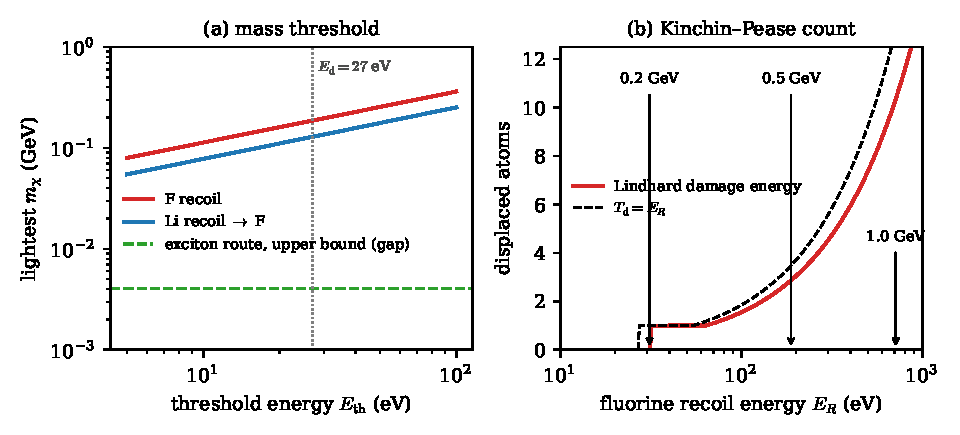
\includegraphics[width=\linewidth]{figures/ch16/fig16_6.pdf}
  \caption{F-center creation in LiF. (a) Lightest dark-matter mass that can create an F center, against the threshold energy of a step: a fluorine recoil above the threshold (red), a lithium recoil that passes the threshold energy to a fluorine neighbor in one head-on collision, transfer fraction 0.788 (blue), and the mass that deposits the band gap, \SI{14.2}{eV}, $\SI{4.0}{MeV}$, an upper bound on the threshold of the exciton route (green, dashed); \cref{eq:1.3-ERmax} with $v_{\mathrm{max}} = \num{2.650e-3}$. Dotted: $E_{\mathrm{d}} = \SI{27}{eV}$, the threshold used in binary-collision simulations of LiF. (b) Atoms displaced by a fluorine recoil in the Kinchin--Pease count with $E_{\mathrm{d}} = \SI{27}{eV}$, with the damage energy of the Lindhard partition for $Z = 9$, $A = 19$ (red; an extrapolation below about \SI{1}{keV}) and with no electronic loss (black, dashed). Arrows: the largest fluorine recoil energy for $\mchi = 0.2$, 0.5 and \SI{1.0}{GeV}, 31, 188 and \SI{711}{eV}.}
  \label{fig:16-lif}
\end{figure}

The number of vacancies a recoil makes follows from two classic estimates. The Lindhard partition splits a recoil of energy $E_R$ into an electronic share $y_LE_R$ and a damage energy $T_{\mathrm{d}} = (1 - y_L)E_R$, with $y_L$ of \cref{eq:16.6-lindhard} (\cref{sec:19.3}). The Kinchin--Pease count of \cref{sec:19.4-count}~\cite[Sect.~II]{cogswell2021passive} then gives no vacancy for $T_{\mathrm{d}} < E_{\mathrm{d}}$, one for $E_{\mathrm{d}} \le T_{\mathrm{d}} < 2E_{\mathrm{d}}$, and $T_{\mathrm{d}}/2E_{\mathrm{d}}$ above. The Lindhard partition and the Kinchin--Pease count are both rough at the energies of sub-GeV recoils. The Lindhard form already misses the measured ionization of silicon recoils of \SI{100}{eV} (\cref{app:E.23}), and its use for a fluorine recoil in a compound is a model choice. The Kinchin--Pease count ignores recombination and the direction dependence of $E_{\mathrm{d}}$. The two estimates set the scale of the yield, and \cref{we:16-fyield} uses them only to set that scale.

\begin{workedexample}{The yield of F centers per keV of fluorine recoil}\label{we:16-fyield}
Take a fluorine recoil of \SI{1}{keV} in LiF. With $Z = 9$ and $A = 19$, \cref{eq:16.6-lindhard} gives $k_L = 0.132$, $\epsilon_L = 0.0683$, $g_L = 2.21$ and $y_L = 0.226$: the recoil gives \SI{226}{eV} to the electrons and leaves a damage energy of \SI{774}{eV}. With $E_{\mathrm{d}} = \SI{27}{eV}$ the Kinchin--Pease count is $774/54 = 14.3$ displaced atoms, and 18.5 if no energy went to the electrons. The count does not say how the displacements divide between the two sublattices. If all displacements are on the anion sublattice, the count gives 14.3 fluorine vacancies per keV, an upper value; an equal share gives 7.2.

A fluorine vacancy becomes an F center only with an electron. The electronic share of \SI{226}{eV} makes at most $226/14.2 = 16$ electron--hole pairs, since each costs at least the gap, so at \SI{1}{keV} the electrons and the vacancies are comparable in number, before trapping and recombination take their share.

The balance between electrons and vacancies changes at the energies that sub-GeV dark matter reaches. A particle of \SI{0.5}{GeV} gives at most \SI{188}{eV}, a damage energy of \SI{155}{eV} and 2.9 displacements, but at most 2.3 pairs. At \SI{0.3}{GeV} the largest recoil is \SI{69}{eV}, about one displacement and at most 0.7 pairs; at \SI{0.2}{GeV}, \SI{31}{eV}, which reaches $T_{\mathrm{d}} = E_{\mathrm{d}}$ only without electronic loss. Near threshold a recoil therefore makes one vacancy and less than one free electron, and the charge factor $p_q$ in \cref{eq:16.6-yield} decides how many vacancies become F centers. The per-keV yield of the first paragraph, 7 to 14 fluorine vacancies, is an upper estimate that the four factors of \cref{eq:16.6-yield} reduce by amounts that no measurement fixes.
\end{workedexample}

\subsection{Bond breaking and cage escape}\label{sec:16.6-bond}

Take a diatomic molecule of atoms with masses $M_1$ and $M_2$ in a molecular solid, and let the dark matter strike atom 1. With the center of mass $\vect{R}_{\mathrm{CM}}$ and the bond vector $\vect{r} = \vect{R}_1 - \vect{R}_2$, the struck atom is at
\begin{equation*}
  \vect{R}_1 = \vect{R}_{\mathrm{CM}} + \frac{M_2}{M_{\mathrm{mol}}}\,\vect{r} = \vect{R}_{\mathrm{CM}} + \frac{\mu_{12}}{M_1}\,\vect{r} ,
\end{equation*}
with $M_{\mathrm{mol}} = M_1 + M_2$ and $\mu_{12} = M_1M_2/M_{\mathrm{mol}}$ the reduced mass of the bond. Assume that the forces of the neighbors act on the center of mass only, and depend neither on the length of the bond nor on its orientation. The Hamiltonian then splits into $H_{\mathrm{CM}} + H_{\mathrm{int}}$, the operators of the two parts commute, and so do their Heisenberg evolutions. The Fourier transform of the self correlation of the struck atom is its response (\cref{eq:D.32-I}). With $\vect{q}_{12} = (\mu_{12}/M_1)\vect{q}$ the kick on the bond vector, the self correlation factorizes,
\begin{equation*}
  \bigl\langle\ee^{-\ii\vect{q}\cdot\vect{R}_1(t)}\,\ee^{\ii\vect{q}\cdot\vect{R}_1}\bigr\rangle = \bigl\langle\ee^{-\ii\vect{q}\cdot\vect{R}_{\mathrm{CM}}(t)}\,\ee^{\ii\vect{q}\cdot\vect{R}_{\mathrm{CM}}}\bigr\rangle\,\bigl\langle\ee^{-\ii\vect{q}_{12}\cdot\vect{r}(t)}\,\ee^{\ii\vect{q}_{12}\cdot\vect{r}}\bigr\rangle ,
\end{equation*}
and a product in time is a convolution in frequency:
\begin{keyresult}[Response of an atom in a molecule]
\begin{equation}
  \begin{gathered}
  S_{11}(\vect{q},\omega) = \int\frac{\dd\omega'}{2\pi}\,S_{\mathrm{CM}}(\vect{q},\omega')\,S_{\mathrm{int}}(\vect{q}_{12},\omega - \omega') , \\
  S_{\mathrm{int}}(\vect{q}_{12},\omega) = 2\pi\sum_f\bigl|\langle f|\ee^{\ii\vect{q}_{12}\cdot\vect{r}}|0\rangle\bigr|^2\,\delta(\omega - E_f + E_0) .
  \end{gathered}
  \label{eq:16.6-conv}
\end{equation}
$S_{\mathrm{CM}}$ is the lattice response of a rigid molecule of mass $M_{\mathrm{mol}}$, and $S_{\mathrm{int}}$ the response of the bond to the kick $\vect{q}_{12}$ on its internal coordinate. The part of $S_{\mathrm{int}}$ with final states above the dissociation limit, $E_f - E_0 > E_{\mathrm{bond}}$, is the response for breaking the bond.
\end{keyresult}
\noindent The hypothesis holds best for molecules that rotate freely in the solid, with an internal motion that does not feel the cage. It fails for the fragments of a broken bond, which move through the cage and collide with its walls; the escape probability below accounts for that failure.

$S_{\mathrm{CM}}$ and $S_{\mathrm{int}}$ are both impulsive at the momenta that break bonds. A classical bond breaks when the kinetic energy $q_{12}^2/2\mu_{12}$ given to the internal motion exceeds $E_{\mathrm{bond}}$, which requires
\begin{equation}
  q \ge q_{\min} = \frac{M_1}{\mu_{12}}\,(2\mu_{12}E_{\mathrm{bond}})^{1/2} ,
  \label{eq:16.6-qmin}
\end{equation}
the threshold of Essig et al.~\cite[Eq.~(3.3)]{essig2017detection}. For H$_2$, with their $E_{\mathrm{bond}} = \SI{4.75}{eV}$, $q_{\min} = \SI{134}{keV}$, and a particle needs $\mchi \ge \SI{25.9}{MeV}$ to transfer it. The bond vibrates at $\omega_{\mathrm{vib}} = \SI{0.546}{eV}$~\cite{huber1979constants}, so the internal recoil parameter $E_{\mathrm{bond}}/\omega_{\mathrm{vib}}$ is 8.7, and the center-of-mass recoil, a few eV against intermolecular phonons of meV, is deep in the impulse regime of \cref{sec:11.4}. In the impulse approximation each factor of \cref{eq:16.6-conv} shifts the deposit by a Doppler term. The center of mass shifts it by $\vect{q}\cdot\vect{P}_{\mathrm{CM}}/M_{\mathrm{mol}}$, which changes the minimum velocity $\omega/q + q/2\mchi$ by $(\langle\omega\rangle_{\mathrm{CM}}/2M_{\mathrm{mol}})^{1/2}$ per standard deviation, $2\times10^{-6}$ for H$_2$ with an assumed $\langle\omega\rangle_{\mathrm{CM}} = \SI{10}{meV}$, against $v_{\mathrm{max}} = \num{2.650e-3}$. The center-of-mass shift does not decide whether the bond breaks and plays no further role. The internal factor shifts the energy given to the bond by $\vect{q}_{12}\cdot\vect{p}_{12}/\mu_{12}$, with $\vect{p}_{12}$ the relative momentum in the ground state, and that shift decides the outcome. In the impulse approximation the bond breaks when
\begin{equation}
  \frac{q_{12}^2}{2\mu_{12}} + \frac{\vect{q}_{12}\cdot\vect{p}_{12}}{\mu_{12}} > E_{\mathrm{bond}} .
  \label{eq:16.6-diss}
\end{equation}
Averaging over the ground state gives the dissociation probability of a kick $\vect{q}$. Essig et al.\ take the ground state of a free rotor, a Gaussian in the bond length $|\vect{r}|$ about its equilibrium value, isotropic in direction~\cite[Eq.~(3.12)]{essig2017detection}. With the harmonic width $(\mu_{12}\omega_{\mathrm{vib}})^{-1/2}$ the projection of $\vect{p}_{12}$ on $\hat{\vect{q}}$ has the root-mean-square value $(\mu_{12}\omega_{\mathrm{vib}}/6)^{1/2}$, \SI{6.53}{keV} or 1.75 times $\alpha m_e$ for H$_2$.

The published rates are limits of \cref{eq:16.6-conv,eq:16.6-diss}. With $S_{\mathrm{CM}}$ the free recoil of the molecule and $\vect{p}_{12} \to 0$, the deposit is $q^2/2M_{\mathrm{mol}} + \mu_{12}q^2/2M_1^2 = q^2/2M_1$, the minimum velocity is $q/2\mu_{\chi1}$, and the rate is the free recoil \cref{eq:11.4-LS} of atom 1 cut at $q_{\min}$, the classical rate of Essig et al.~\cite[Eq.~(4.3)]{essig2017detection}. Their quantum rate keeps the spread of the ground state, with plane-wave final states whose internal momentum is set by the energy above the dissociation limit, the improved Born approximation~\cite[Eqs.~(3.11), (3.17), (4.5)]{essig2017detection}. In that approximation the bond breaks when $|\vect{q}_{12} + \vect{p}_{12}|^2/2\mu_{12} > E_{\mathrm{bond}}$. The Born condition differs from \cref{eq:16.6-diss} by the initial kinetic energy of the bond, $\langle p_{12}^2\rangle/2\mu_{12} = \omega_{\mathrm{vib}}/4 = \SI{0.136}{eV}$ for H$_2$: the Born form counts the final kinetic energy of the fragments from zero, the impulse form counts the energy the kick adds.

\begin{limitbox}[Color-center creation and bond breaking][lim:16.6a]
The published color-center rate is the free nuclear recoil \cref{eq:11.4-LS} cut by a step at the displacement threshold, $\Theta(E_R - E_{\mathrm{d}})$~\cite[Eqs.~(1), (2), (5), (7)]{budnik2018direct}. The published classical bond-breaking rate is the free recoil of the struck atom cut at $q_{\min}$ of \cref{eq:16.6-qmin}~\cite[Eqs.~(3.3), (4.3)]{essig2017detection}.
\par\smallskip
{\centering
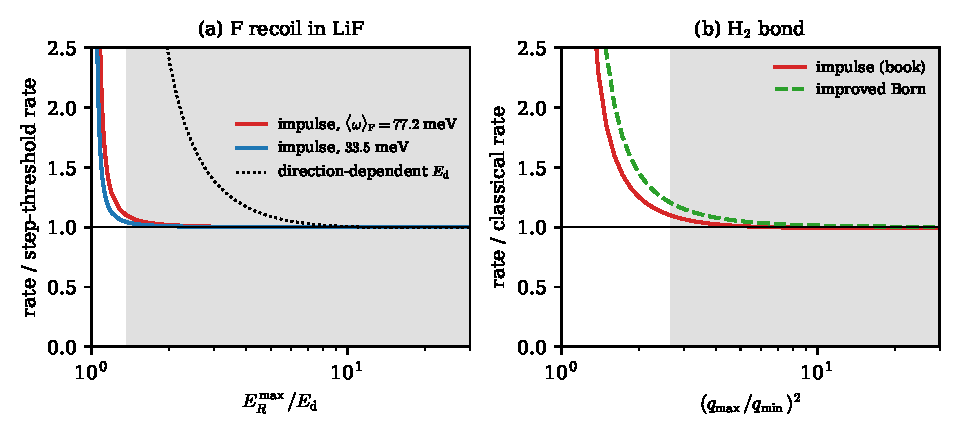
\includegraphics[width=\linewidth]{figures/ch16/limit16_6a.pdf}
\captionof{figure}{Rates from the impulse response of the bound target divided by the published forms, heavy mediator, standard halo, $T = 0$. (a) Fluorine recoils in LiF with $E_{\mathrm{d}} = \SI{27}{eV}$, against the ratio of the largest recoil energy to the threshold: \cref{eq:16.6-ccrate} with the yield a step at $\omega = E_{\mathrm{d}}$, for $\langle\omega\rangle_{\mathrm{F}} = \SI{77.2}{meV}$ (red, the top of the LiF optical band, an upper value) and \SI{33.5}{meV} (blue). Dotted: the direction-dependent threshold $E_{\mathrm{d}}(1 + a\sin4\theta\cos4\varphi)^2$ with $a = 0.4$, recoil directions isotropic in the crystal, divided by the step at $E_{\mathrm{d}}$. (b) H$_2$ as a free rotor: \cref{eq:16.6-conv} with \cref{eq:16.6-diss} over the Gaussian ground state (red) and with the improved Born condition (green, dashed), against $(q_{\max}/q_{\min})^2$, $q_{\max} = 2\mu_{\chi1}v_{\mathrm{max}}$. Gray: the red curve within \SI{10}{\percent} of one, $E_R^{\max} \ge 1.36\,E_{\mathrm{d}}$ ($\mchi \ge \SI{0.218}{GeV}$) in (a) and $(q_{\max}/q_{\min})^2 \ge 2.65$ ($\mchi \ge \SI{42.9}{MeV}$) in (b).}\label{fig:16-limit-cc}
\par}
\smallskip
Closer to threshold the color-center and bond-breaking rates both depend on the zero-point motion of the struck nucleus or bond and stay nonzero below the classical endpoint, and at every mass they still lack the yield factors of \cref{eq:16.6-yield} and the escape probability of the fragments of a bond, which multiply both curves.
\end{limitbox}

In \cref{lim:16.6a} the Doppler width changes the LiF rate by less than \SI{2}{\percent} once the largest recoil energy exceeds twice the threshold, and with the Doppler width the rate reaches the step-form rate for $E_R^{\max} = 1.1\,E_{\mathrm{d}}$ at a mass \SI{1.4}{\percent} lower. The directional structure of the threshold matters more: with the angular model of Budnik et al.\ the rate stays more than \SI{10}{\percent} away from the step value up to $E_R^{\max} = 4.8\,E_{\mathrm{d}}$, or $\mchi = \SI{0.41}{GeV}$, because the threshold surface reaches down to $0.36\,E_{\mathrm{d}}$. For H$_2$ the impulse rate equals the classical rate of $\mchi = \SI{27.2}{MeV}$ already at \SI{22.8}{MeV}, a shift of the mass scale by a factor 0.84; the improved Born rate does so at \SI{20.3}{MeV}, a factor 0.75.

A broken bond is not yet a signal. In a solid the two fragments start inside the cage of their neighbors, and they recombine unless they escape it; this recombination inside the cage is the cage effect of photochemistry. The rate of separated fragments is the rate of dissociating seeds times the escape probability $p_{\mathrm{esc}}(E_{\mathrm{int}},\hat{\vect{r}})$, which depends on the energy $E_{\mathrm{int}}$ the fragments share above the dissociation limit and on the direction of the bond relative to the cage. Electronic deposits break bonds as well: an excitation into a repulsive state, the antibonding $\sigma^*$ surface of the bond, dissociates the molecule without any nuclear kick, at the electronic thresholds of the molecular crystals of \cref{sec:16.4}. Neither $p_{\mathrm{esc}}$ nor the dissociation yields of these electronic states have been quantified at the momenta and temperatures of a dark-matter search.

\subsection{Measured yields and single-center readout}\label{sec:16.6-yields}

Of the inputs to \cref{eq:16.6-yield}, the displacement threshold is the one with measurements, and these fix only its lowest point. Electron irradiation of silicon sees damage set in at $12.9 \pm \SI{0.6}{eV}$, where density-functional molecular dynamics puts the minimum of $E_{\mathrm{d}}(\hat{\vect{r}})$ (\cref{sec:7.4}). The shape of $p_{\mathrm{FP}}$ above the minimum is a computed quantity: the defect probability becomes nonzero below the average threshold and approaches one only at two to three times the average threshold~\cite[Sect.~II]{cogswell2021passive}. In materials where an interstitial recombines with its own vacancy a direction-resolved threshold is not even well defined (\cref{app:E.11}). For ionic crystals the measured responses are those of dense tracks at room temperature: fast neutrons, $\gamma$ rays of $^{60}$Co, and the $\alpha$ and triton tracks of neutron capture on $^6$Li~\cite{araujo2026nuclear}. The aggregates that LiF forms along these dense tracks are stable for months in vacuum at room temperature and anneal away at \SI{350}{\celsius}~\cite[Sect.~III]{araujo2026nuclear}. None of these measurements isolates a single recoil of tens to hundreds of eV, and none is made at millikelvin temperatures.

A single-center readout at millikelvin temperatures must work without aggregation. A sub-GeV recoil makes one to three vacancies (\cref{we:16-fyield}), and at \SI{10}{mK} they do not move, so the emitting aggregates read in LiF tracks do not form and the readout must find a single F center. In LiF that center has no observed luminescence~\cite{guerreroperez2025first}, so it must be found through its absorption near \SI{5.1}{eV}, in the ultraviolet, or converted into a state that emits. For an emitting center in a light-guiding rod, Budnik et al.\ estimate $5\times10^5$ detected photons in \SI{e3}{s} and a detection limit of about one new center among $10^5$ existing ones~\cite[footnote~1]{budnik2018direct}. The existing centers set the background. Commercial crystals are not certified below a defect concentration of $10^{-9}$, and annealing at up to \SI{1000}{\celsius} removes many of the existing centers~\cite{budnik2018direct}; fluorescence measurements of LiF put an upper limit of $10^{-12}$ to $10^{-10}$ on the centers present before irradiation~\cite{cogswell2021passive}. At millikelvin temperatures the readout light must also deposit less heat than the detector tolerates; none of these estimates addresses this heat load.

Four yields remain open at millikelvin temperatures: the conversion $p_{\mathrm{FH}}$ of a self-trapped exciton into a Frenkel pair, the survival $p_{\mathrm{surv}}$ of a close pair with the charge factor $p_q$ at recoil energies of tens to hundreds of eV, the efficiency $f_{\mathrm{opt}}$ of reading a single center, and the escape $p_{\mathrm{esc}}$ of the fragments of a bond with the yields of repulsive electronic states. Each can be measured directly. Neutrons scattered at a tagged angle in LiF at \SI{10}{mK} give recoils of known energy, and counting single F centers per tagged recoil measures the product $p_{\mathrm{FP}}p_{\mathrm{surv}}p_qf_{\mathrm{opt}}$ as a function of $E_R$. X-rays of \SI{5.9}{keV} absorbed at millikelvin temperatures give $p_{\mathrm{FH}}$ from the F-center yield per absorbed energy together with the quenching of the exciton luminescence. The photodissociation quantum yield of a molecular crystal at millikelvin temperatures, with the fragments detected by infrared absorption, gives $p_{\mathrm{esc}}$.
